\documentclass[12pt,fleqn]{article}\usepackage{../../common}
\begin{document}
Materyel Mekaniği - 6

Direk Direngenlik Metotu (Direct Stiffness Method)

Direngenlik metotunu anlamak icin direngenlik matrisi kavramini islemek
gerekir. Bu konuya biraz [2]'de degindik. Bir oge grubunun, sistemin direngenlik
matrisi dugumsel yer degisimler $d$ ile dugumsel kuvvetler $F$'yi ilintilendiren
bir $K$ matrisidir, oyle ki [1, sf. 34]

$$
F = K d
$$

esitligi gecerlidir. Alttaki gibi bir sistem olsun,

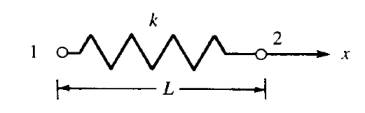
\includegraphics[width=15em]{phy_020_strs_06_03.jpg}

Sistemde bir yay goruluyor, bu yay uzerinde iki tane dugum noktasi sectik,
onlari takip edecegiz, dugum 1 ve 2. Dugumlerdeki yer degisimler $u_1,u_2$
olsun, yaydaki toplam degisimo $\delta = u_1 - u_2$. Uygulanan kuvvet $T$
ise bir sabit $k$ uzerinden $T = k \delta$ esitligi ortaya atilabilir.

Direngenlik matrisine gelirsek, sistemdeki tum yer degisimleri soyle gosterebiliriz,

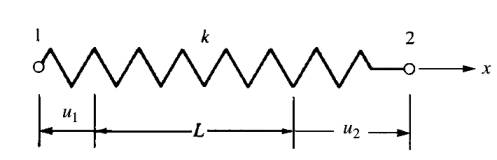
\includegraphics[width=15em]{phy_020_strs_06_04.jpg}

Sag ucta yay $T$ kuvveti ile cekiliyorsa, bu durum sol ucta $-T$ tepkisel
kuvvete sebep olur. Ayrica $u_1$'in sol yonu isaret ettigine dikkat, cunku yer
degisimin yonu pozitif yonun tersinde, yaydaki takip edilen nokta baslangic
aninin sol tarafinda kaliyor, bu sebeple yon eksi.

$$
f_{1x} = -T, \quad f_{2x} = T
$$

Hepsini bir araya koyarsak

$$
T = -f_{1x} = k (u_2 - u_1)
$$

$$
T = f_{2x} = k (u_2 - u_1)
$$


Bir yay sistemini temsil edebilecek direngenlik matrisini nasıl
bulabileceğimizin bir örneğini [2]'de gördük. Alternatif bir
teknik olarak üstdüşüm / üst üste koyma (superposition) tekniğini
işleyelim [1, sf. 38]. 

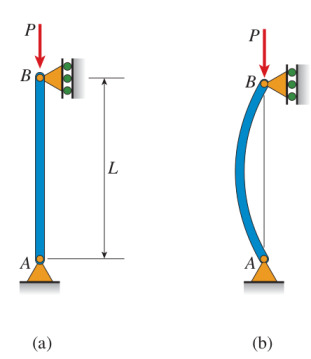
\includegraphics[width=20em]{phy_020_strs_06_02.jpg}


$$
\begin{array}{cc} & \begin{array}{ccc} a & b & c \end{array} \\ &
\left(
\begin{array}{ccc}
.1 & .1 & 0 \\
.4 & 1 & 0 \\
.8 & 0 & .4
\end{array}
\right)
\end{array}
$$





[devam edecek]


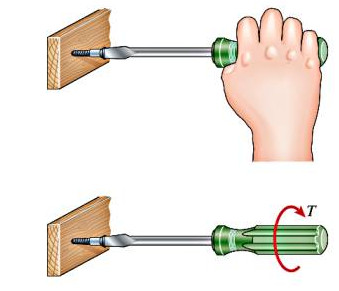
\includegraphics[width=20em]{phy_020_strs_06_01.jpg}


Kaynaklar

[1] Logan, {\em A First Course in the Finite Element Method}

[2] Bayramlı, {\em Hesapsal Bilim, Ders 1-8}

\end{document}
